\section{Speed evaluation}

\subsection{Overall speed}

The full pipeline took 42s to process a video composed of 1000 frames, thus resulting in a speed of 38 FPS, higher than what was required.
To avoid waiting times due to the camera framerate, these measurements were computed by using a video previously captured and saved as set of frames on the disk.

\subsection{Speed of the pipeline steps}

As visible in figure~\ref{fig:speed:all-pipeline}, the process is 2.3x as fast as the initial SMA-RTY implementation, which was already faster than the provided Matlab script.
Naturally, the last step to complete is the last one of the pipeline, the \link*: however, as the next sections will show, the bottleneck is in the \locate* step.

\begin{figure}
	\centerline{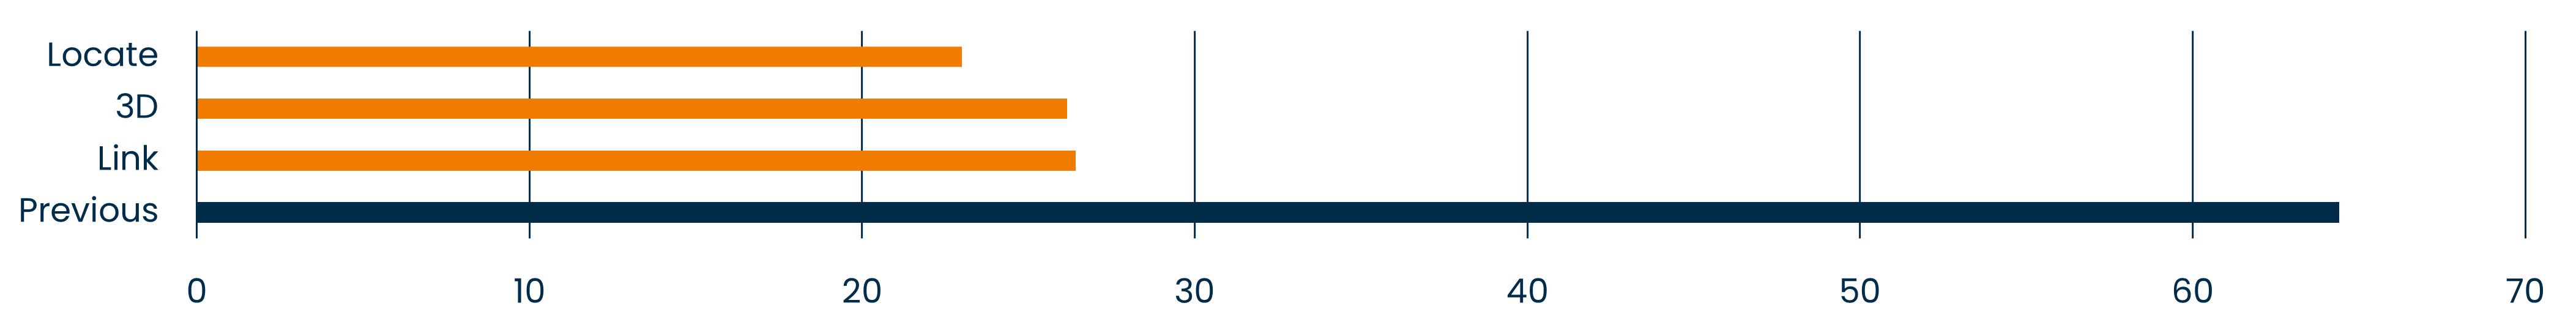
\includegraphics[width=\textwidth]{images/speed/overall-speed.png}}
	\caption{\centering The time required (in seconds) by the different pipeline steps to process a 1000-frames video}
	\label{fig:speed:all-pipeline}
\end{figure}

\subsubsection{\locate* step}

As shown in figure~\ref{fig:speed:locate}, the \locate* step was always fully operational.
The main bottleneck is the loading of the images from the HDD to the RAM for processing.

\begin{figure}
	\centerline{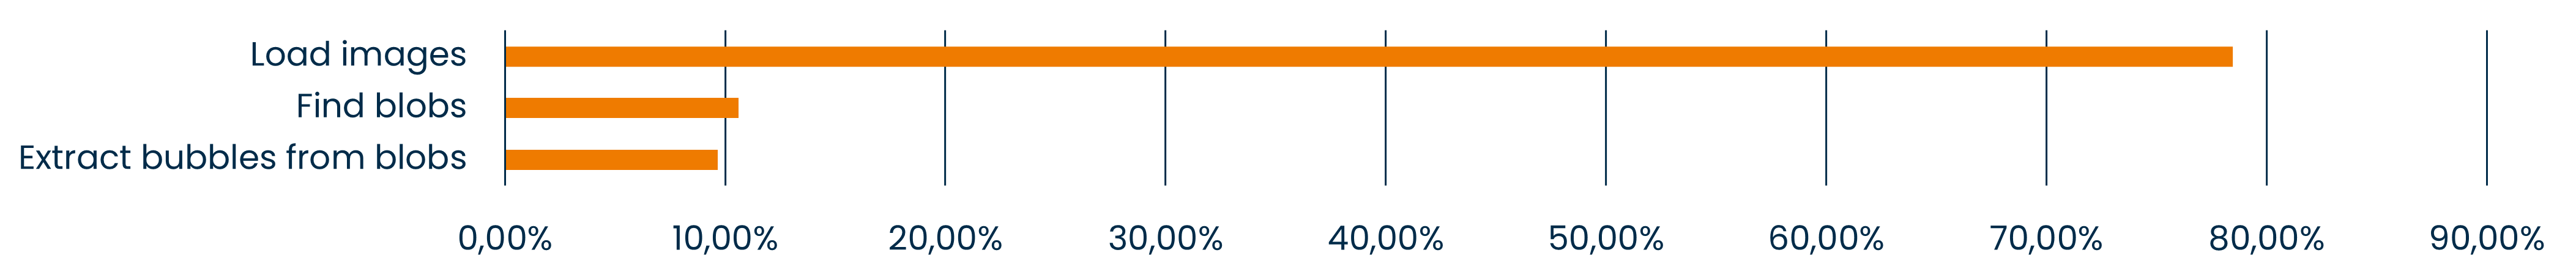
\includegraphics[width=\textwidth]{images/speed/locate.png}}
	\caption{\centering Distribution of how the \locate* step spent its execution time}
	\label{fig:speed:locate}
\end{figure}

\subsubsection{\match* step}

The \match* step, as visible in figure~\ref{fig:speed:match}, requires to spend a small amount of time waiting for the \locate* data.
This means that the \match* step is not the bottleneck.
The waiting time is however not extensive, indicating that even small slowdowns may make this step the bottleneck, affecting the whole pipeline performance.

\begin{figure}
	\centerline{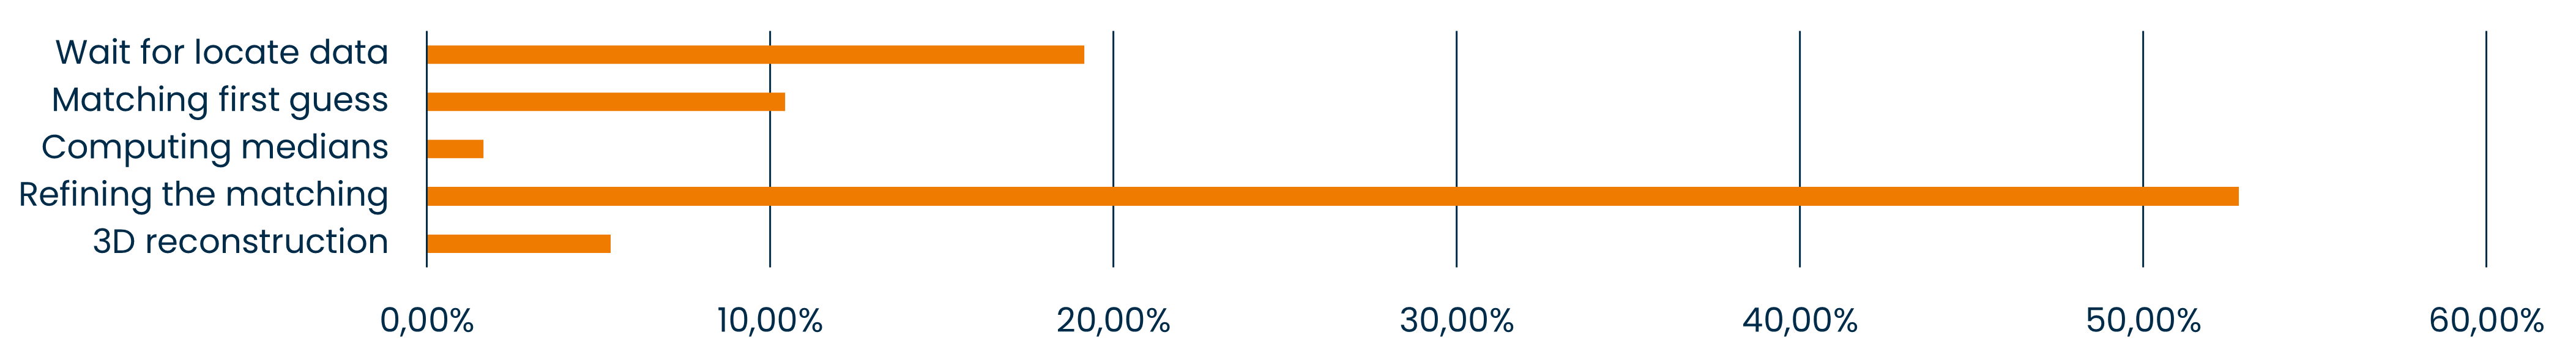
\includegraphics[width=\textwidth]{images/speed/matching.png}}
	\caption{\centering Distribution of how the \match* step spent its execution time}
	\label{fig:speed:match}
\end{figure}

\subsubsection{\link* step}

Figure~\ref{fig:speed:link} shows that most of the time the \link* step is idling, waiting for new inputs to be processed.
This indicates that it is far from being the bottleneck, and potentially more complex algorithm could be used instead, if they provided better results.

\begin{figure}[H]
	\centerline{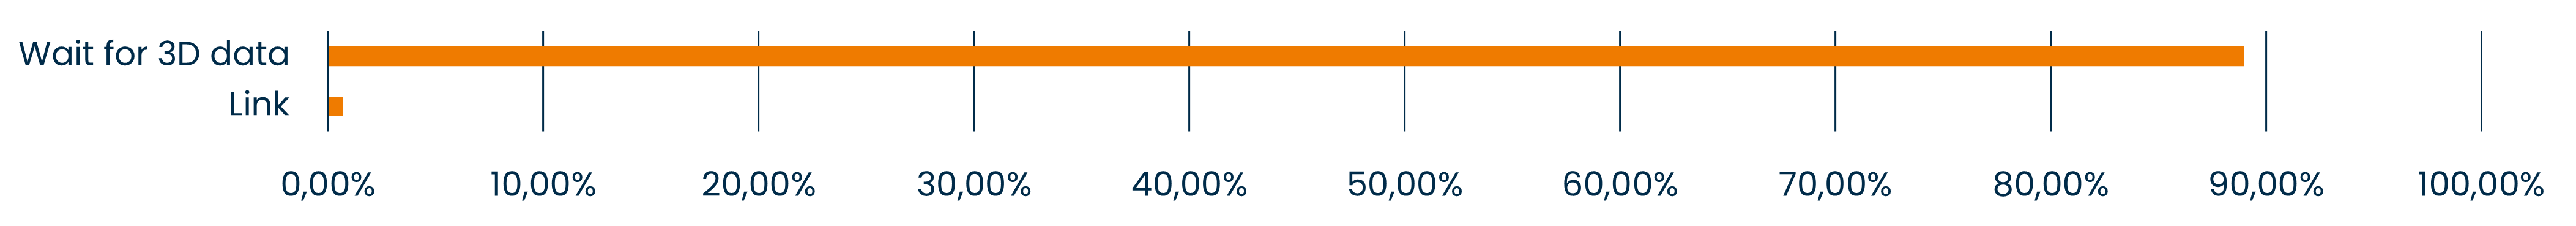
\includegraphics[width=\textwidth]{images/speed/link.png}}
	\caption{\centering Distribution of how the \link* step spent its execution time}
	\label{fig:speed:link}
\end{figure}
